\section{Microcontroller}

\begin{remark}
    \begin{itemize}
        \item Microcontroller
        \item System Bus
        \item Digital Logic Basics
        \item Synchronous Bus
        \item Control and Status Registers
        \item Address Decoding
        \item Slow Slaves (Peripherals)
        \item Bus Hierarchies
        \item Accessing Control Registers in C
        \item Conclusions
    \end{itemize}
\end{remark}

\begin{theorem}{Embedded Systems}
    \begin{itemize}
        \item low cost (usb sticks, consumer electronics)
        \item low power (sensor networks, mobile devices)
        \item small size (smart cards, wearables)
        \item real time (anti-lock brakes, process control)
        \item reliability (medical devices, automotive)
        \item extreme environment (space, automotive)
    \end{itemize}
\end{theorem}

\begin{concept}{Single Chip Solution} 
    $\Rightarrow$ CPU with integrated memory and peripherals
    
    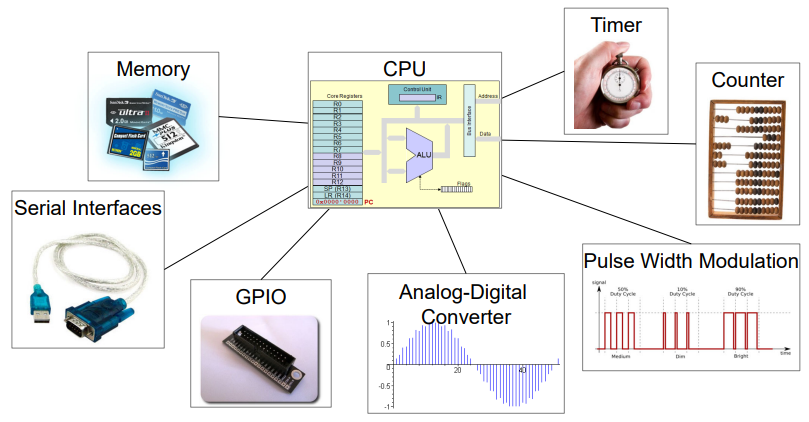
\includegraphics[width=\linewidth]{single_chip_solution.png}
\end{concept}

\begin{definition}{Peripherals}
    \begin{itemize}
        \item configurable hardware blocks of a microcontroller
        \item accepts a specific task from the CPU, executes task and returns result (status, e.g. task completion, error)
        \item oftentimes interfaces to the outside world\\
        many (not all) interact with external MCU pins (grey things very right side of image)
        \item examples: GPIO, UART, SPI, ADC...
    \end{itemize}
    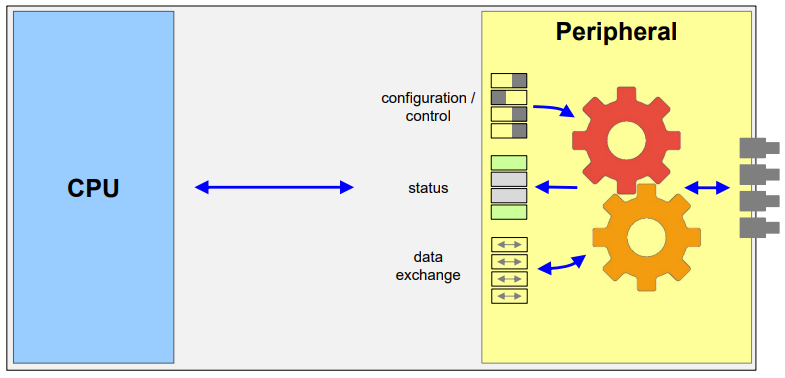
\includegraphics[width=\linewidth]{peripherals1.png}
\end{definition}

\begin{definition}{Peripheral Registers}
    the CPU controls and monitors Peripherals through registers
    \begin{itemize}
        \item Registers are arrays of flip-flops (storage elements with two states, i.e. 0 or 1)
        \item Each flip-flop stores one bit of information
        \item CPU writes to and reads from registers
    \end{itemize}
    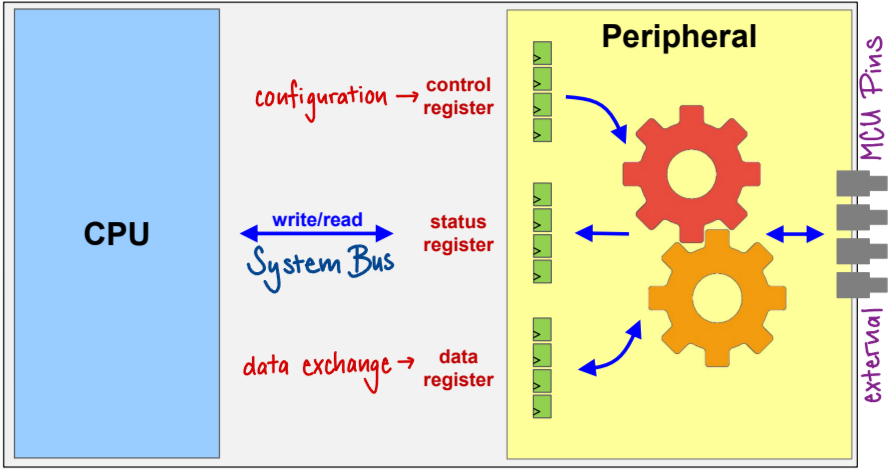
\includegraphics[width=\linewidth]{peripherals_registers.png}

    \tcblower
    A Peripheral typically has multiple registers that can be categorized as:
    \begin{itemize}
        \item \textbf{Control Registers} \\
        enable CPU to configure the peripheral
        \item \textbf{Status Registers} \\
        enable CPU to monitor the peripheral
        \item \textbf{Data Registers} \\
        enable CPU to exchange data with the peripheral
    \end{itemize}
\end{definition}

\begin{definition}{Memory-mapped Peripheral Registers}
    Distinction between LEDs and DIP switches on the CT-Board:
    \begin{itemize}
        \item Control register $\rightarrow$ controls states of LEDs
        \item Status register $\rightarrow$ monitors states of DIP switches
    \end{itemize}
    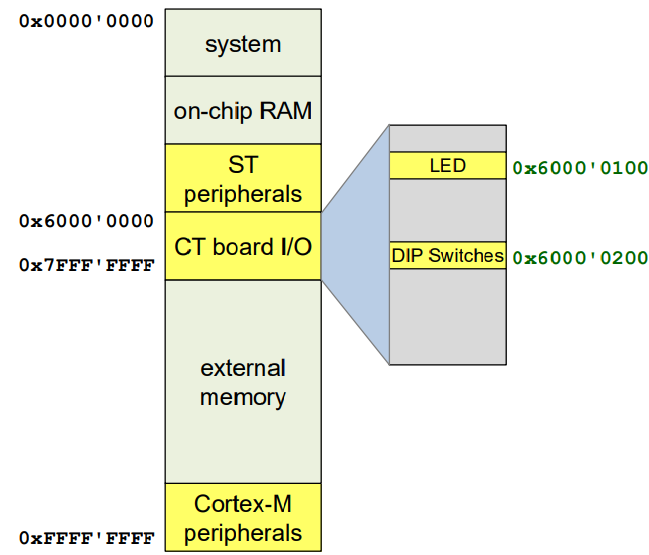
\includegraphics[width=\linewidth]{registers_leds_dipswitches.png}
\end{definition}

\begin{concept}{CPU access to individual peripheral registers}
    \begin{itemize}
        \item ARM \& STM map the peripheral registers into
        the memory address range
        \item Reference Manual shows the defined addresses
    \end{itemize}
    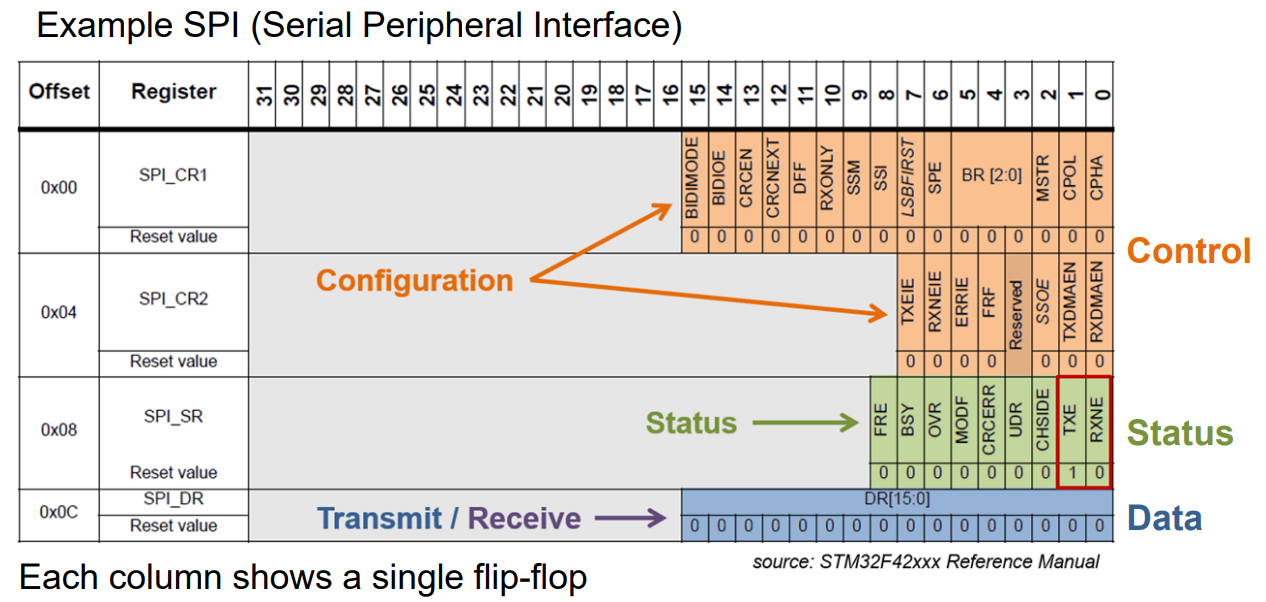
\includegraphics[width=\linewidth]{example_SPI_cpu_access.png}

    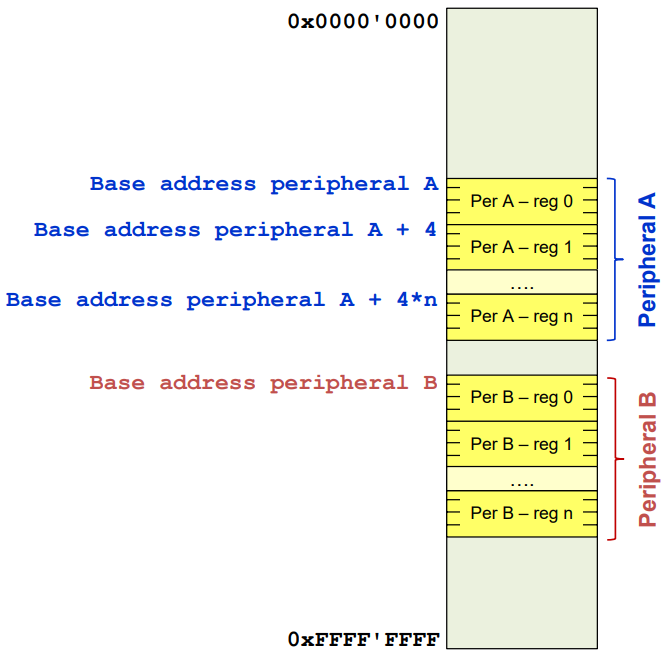
\includegraphics[width=\linewidth]{peripheral_registers_cpu_access.png}

\end{concept}

\begin{examplecode}{Accessing control registers in C}
    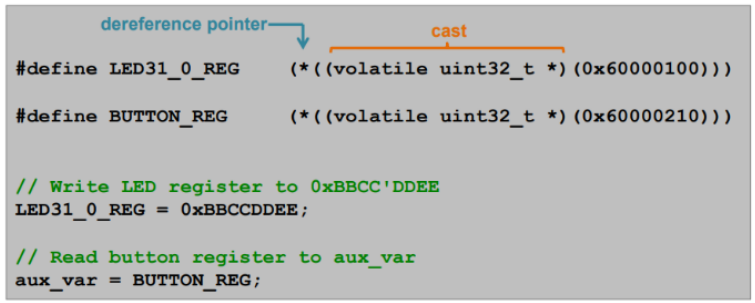
\includegraphics[width=\linewidth]{accessing_control_registers_in_C.png}
\end{examplecode}

\begin{concept}{CPU read/write to peripheral registers}
    How does the CPU write to and read from peripheral registers?
    \begin{itemize}
        \item CPU reads/writes to peripheral registers
        \item CPU uses memory-mapped I/O to access peripheral registers
        \item CPU uses load/store instructions to access peripheral registers
    \end{itemize}
    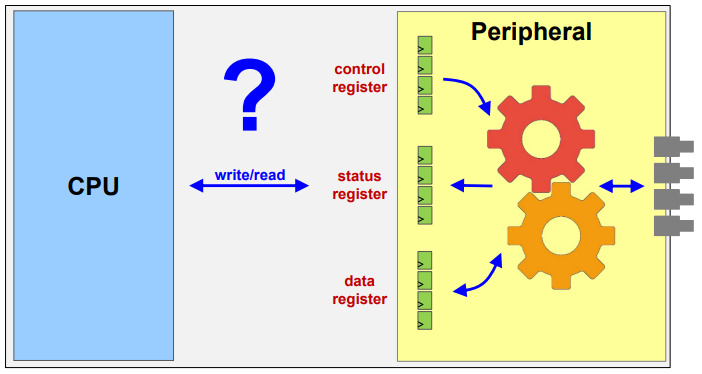
\includegraphics[width=\linewidth]{read_write_cpu_peripheral_registers.png}

    $\Rightarrow$ System Buses
\end{concept}

\begin{example2}{STM32 Microcontroller}
    with CPU, on-chip memory, and peripherals interconnected through the system bus(es)

    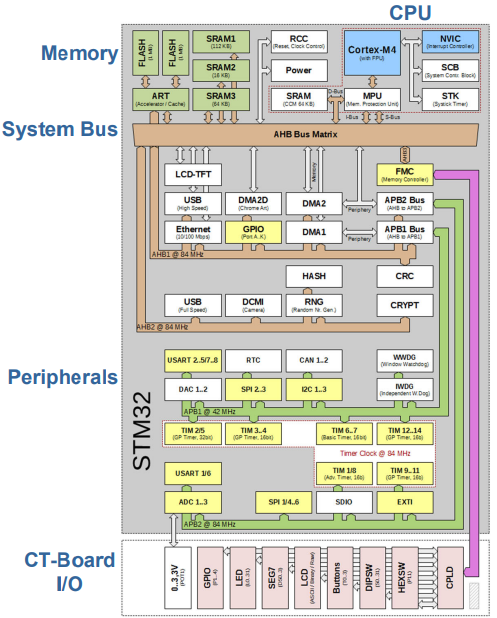
\includegraphics[width=\linewidth]{stm32_example.png}

    A distributed system with parallel (simultaneous) processing of data in many peripherals. All under the supervision of the CPU.
\end{example2}

\begin{remark}
    Note: ARM calls their system buses AHB (ARM High-performance Bus) and APB (ARM
    Peripheral Bus). On complex chips, it is state-of-the-art to partition the system bus into
    multiple interconnected buses.
\end{remark}

\begin{example2}{CT Board with STM32 Microcontroller and Buses}
    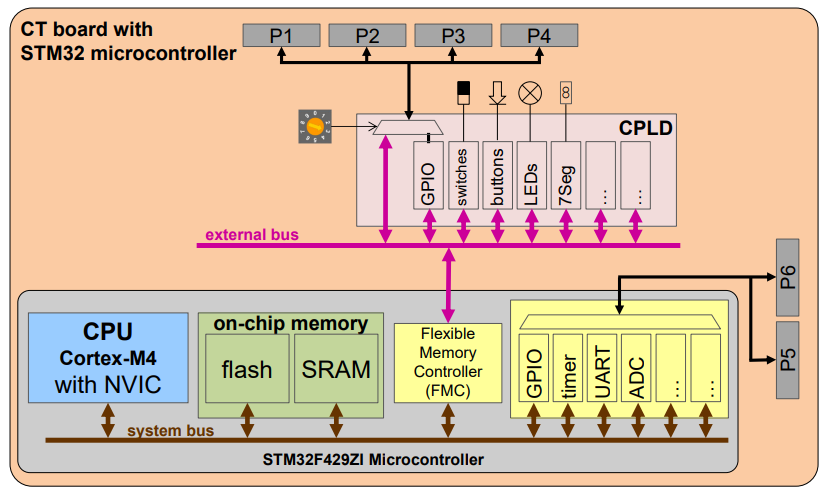
\includegraphics[width=\linewidth]{ctboard_with_stm32.png}
\end{example2}

\begin{definition}{System Bus}
    \begin{itemize}
        \item Interconnects CPU with memory and peripherals
        \item CPU acts as master: initiating and controlling all transfers
        \item Peripherals and memory act as slaves: responding to requests from the CPU
        \item System bus is a shared resource
    \end{itemize}
    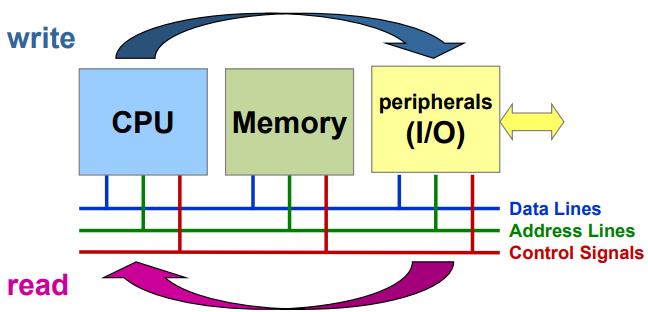
\includegraphics[width=\linewidth]{system_bus.png}
\end{definition}

\begin{concept}{Bus Specification}
    \begin{itemize}
        \item \textcolor{darkblue}{\textbf{Protocol and operations}}
        \item \textcolor{darkred}{\textbf{Signals}}
        \begin{itemize}
            \item Number of Signals
            \item Signal descriptions
        \end{itemize}
        \item \textcolor{darkgreen}{\textbf{Timing}}
        \begin{itemize}
            \item Frequency
            \item Setup and hold times
        \end{itemize}
        \item \textcolor{darkpurple}{\textbf{Electrical properties}} (not in exam)
        \begin{itemize}
            \item Drive strength
            \item Load
        \end{itemize}
        \item \textcolor{darkorange}{\textbf{Mechanical requirements}} (not in exam)
    \end{itemize}
\end{concept}

\begin{theorem}{Signal Groups}
    \begin{itemize}
        \item \textcolor{darkblue}{\textbf{Data lines}}
        \begin{itemize}
            \item Bidirectional (read/write)
            \item Number of lines $\rightarrow$ data bus width \\(8, 16, 32, 64 parallel lines of data)
            \item Example: Cortex-M has 32 address lines $\rightarrow$ 4GB address space $\rightarrow$ $0x00000000$ to $0xFFFFFFFF$
        \end{itemize}
        \item \textcolor{darkgreen}{\textbf{Address lines}}
        \begin{itemize}
            \item Unidirectional: from Master to slaves
            \item Number of lines $\rightarrow$ size of address space
        \end{itemize}
        \item \textcolor{darkred}{\textbf{Control signals}}
        \begin{itemize}
            \item Control read/write direction
            \item Provide timing information
            \item Chip select, read/write, etc.
        \end{itemize}
    \end{itemize}
    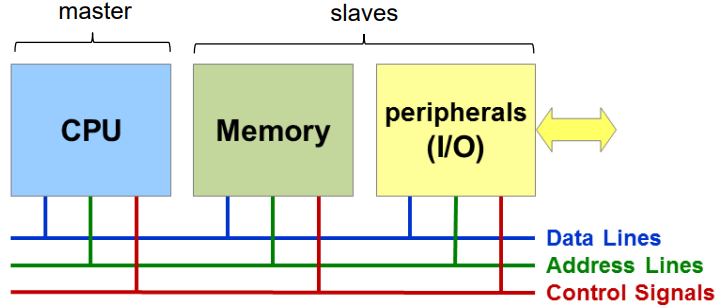
\includegraphics[width=\linewidth]{master_slave_signal_groups.png}
\end{theorem}

\begin{theorem}{Bus Timing Options}

    \begin{minipage}{0.7\linewidth}
    \textbf{Synchronous}
    \begin{itemize}
        \item \textcolor{blue}{Master} and \textcolor{darkcorn}{slaves} use a common clock\\
        \small{Often a dedicated clock signal from master to slave, but clock can also be encoded in a data signal}
        \item \normalsize Clock edges control bus transfer on both sides
        \item Used by most on-chip buses
        \item Off-chip: DDR and synchronous RAM
    \end{itemize}
    \end{minipage}
    \begin{minipage}{0.29\linewidth}
        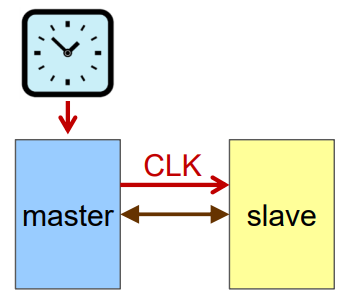
\includegraphics[width=\linewidth]{synchronous_bus_timing.png}
    \end{minipage}

    \begin{minipage}{0.7\linewidth}
    \textbf{Asynchronous}
    \begin{itemize}
        \item \textcolor{darkcorn}{Slaves} have no access to clock of the \textcolor{blue}{master}
        \item Control signals carry timing information to allow synchronization
        \item Widely used for low data-rate off-chip memories
        $\rightarrow$ parallel flash memories and \\ asynchronous RAM
    \end{itemize}
    \end{minipage}
    \begin{minipage}{0.29\linewidth}
        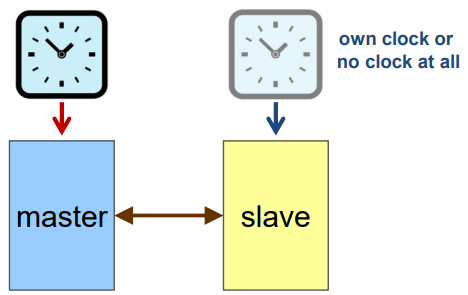
\includegraphics[width=\linewidth]{asynchronous_bus_timing.png}
    \end{minipage}
\end{theorem}

\begin{corollary}{Multiple devices driving the same data line}\\
    What if one device drives a logic 1 (Vcc) and another device drives a logic 0 (Gnd)?\\
    $\Rightarrow$ Electrical short circuit! $rightarrow$ bus contention ("Streitigkeit")\\
    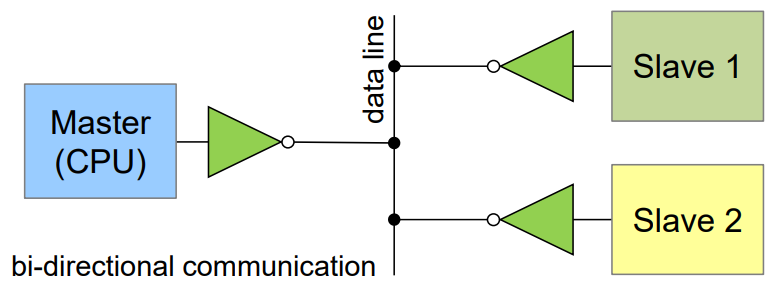
\includegraphics[width=\linewidth]{bus_contention.png}\\
    \small{Figure only shows output paths, input paths are not shown.}

    \tcblower
    CPU defines who drives the data bus at which moment in time:
    \begin{itemize}
        \item \texttt{write} CPU drives bus $rightarrow$ all slave drivers disconnected
        \item \texttt{read} CPU releases bus $rightarrow$ one slave drives bus (selected through values on address lines, other slave drivers disconnected)
    \end{itemize}
    
    Electrically disconnecting a driver is called \textbf{tri-state} or \textbf{high-impedance} (Hi-Z) state. (switch)
    
    \textcolor{pink}{textbf{CHECK IF CORRECT}}
\end{corollary}

\begin{definition}{Slow Slaves}\\
    Wait states are inserted to slow down the CPU to match the speed of the slowest peripheral (depending on the address of an access)

    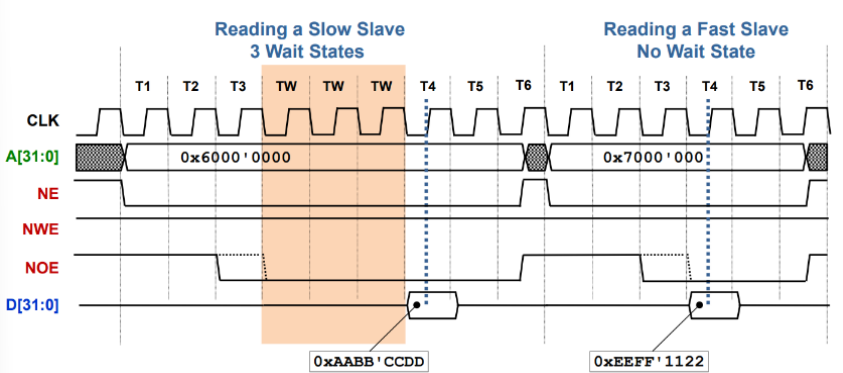
\includegraphics[width=\linewidth]{slow_slaves.png}    
\end{definition}

\begin{formula}{Block Diagram}
    \begin{itemize}
        \item Address lines [31:0]
        \item Data lines [31:0]
        \item Control signals
        \begin{itemize}
            \item CLK $\rightarrow$ clock
            \item NE $\rightarrow$ Not enable
            \item NWE $\rightarrow$ Not write enable
            \item NOE $\rightarrow$ Not output enable
        \end{itemize}
    \end{itemize}
    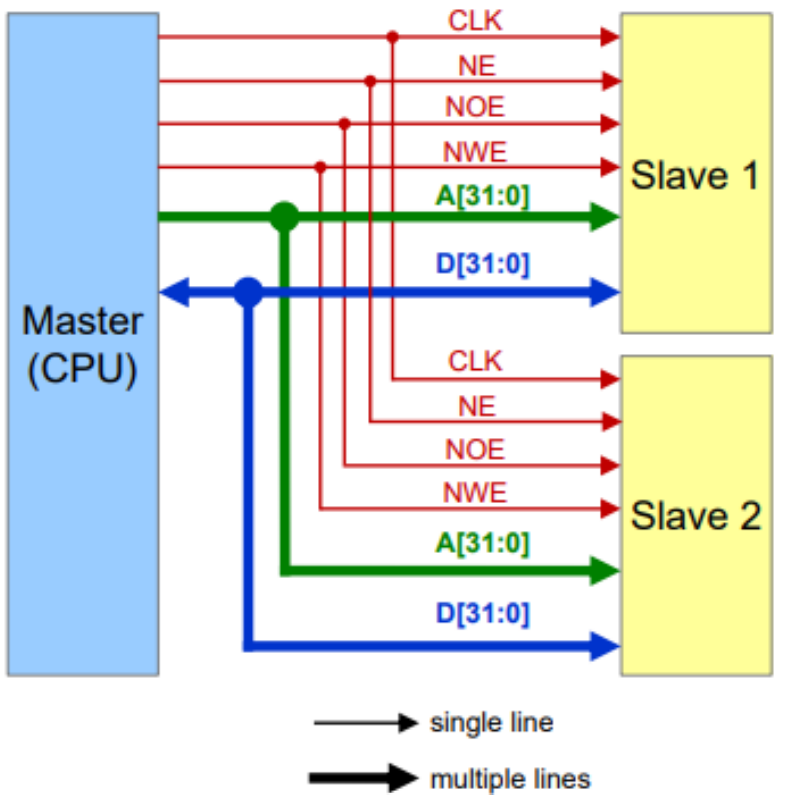
\includegraphics[width=\linewidth]{block_diagramm.png}
\end{formula}

\begin{concept}{Control Bits}
    \begin{itemize}
        \item Allow CPU to configure Slaves
        \item CPU writes to register bit to configure Slave
        \item Slave uses output of register bit to configure itself
        \item Example: SPI Slave Select (SS) bit
        \item Usually read/write access to control bits
    \end{itemize}
\end{concept}

\begin{concept}{Status Bits}
    \begin{itemize}
        \item Allow CPU to monitor Slaves
        \item CPU reads register bit to monitor Slave
        \item Slave uses input of register bit to monitor itself (Slave writes to register bit)
        \item Example: SPI Busy bit
        \item Usually read-only access to status bits
    \end{itemize}
\end{concept}

\begin{formula}{Timing Diagram}
    \begin{itemize}
        \item \texttt{write} \textcolor{darkblue}{D[:]} to \textcolor{darkgreen}{A[:]} $\rightarrow$ \textcolor{darkred}{NE, NWE} = 0
        \item \texttt{read} \textcolor{darkblue}{D[:]} from \textcolor{darkgreen}{A[:]} $\rightarrow$ \textcolor{darkred}{NE, NOE} = 0
    \end{itemize}
    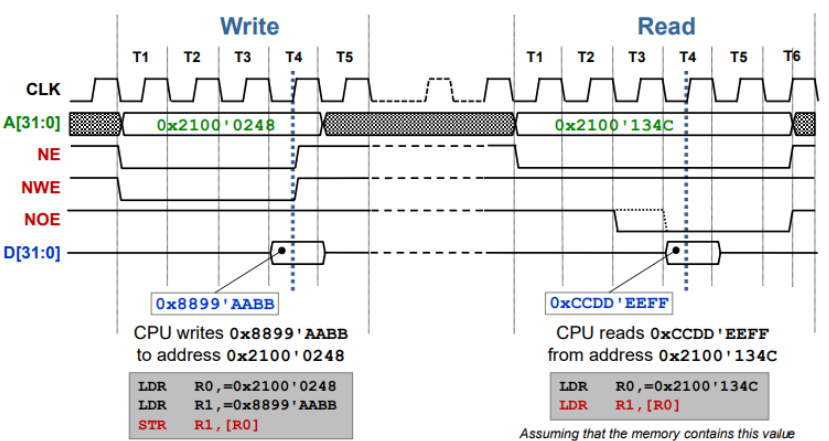
\includegraphics[width=\linewidth]{timing_diagram.png}
\end{formula}

\begin{theorem}{Bus Access Size}
    is determined by the NBL (0-3) (No Byte Line) signals
    \begin{itemize}
        \item NBL = 1 $\rightarrow$ Byte used for Read/Write
        \item NBL = 00
        \item NBL[0:3] = 0011 $\rightarrow$ Read Halfword
        \item NBL[0:3] = 1111 $\rightarrow$ Read Word
    \end{itemize}
    \textcolor{pink}{\textbf{CHECK IF CORRECT}}
\end{theorem}

\begin{definition}{Address Decoding}\\
    Interpretation of address line values. See whether bus access targets a particular address or address range.
    \begin{itemize}
        \item CPU uses address lines to select a peripheral
        \item Each peripheral has a unique address range
        \item Address decoding logic generates a chip select signal for each peripheral
    \end{itemize}

    \textbf{Full Address Decoding}
    \begin{itemize}
        \item All address lines are decoded
        \item A control register can be accessed at exactly one location
        \item 1:1 mapping: A unique address maps to a single hardware register
    \end{itemize}

    \textbf{Partial Address Decoding}
    \begin{itemize}
        \item Only a subset of address lines are decoded
        \item A control register can be accessed at multiple locations
        \item 1:n mapping: Multiple addresses map to the same hardware register
        \item Map a hardware register to multiple addresses
    \end{itemize}
    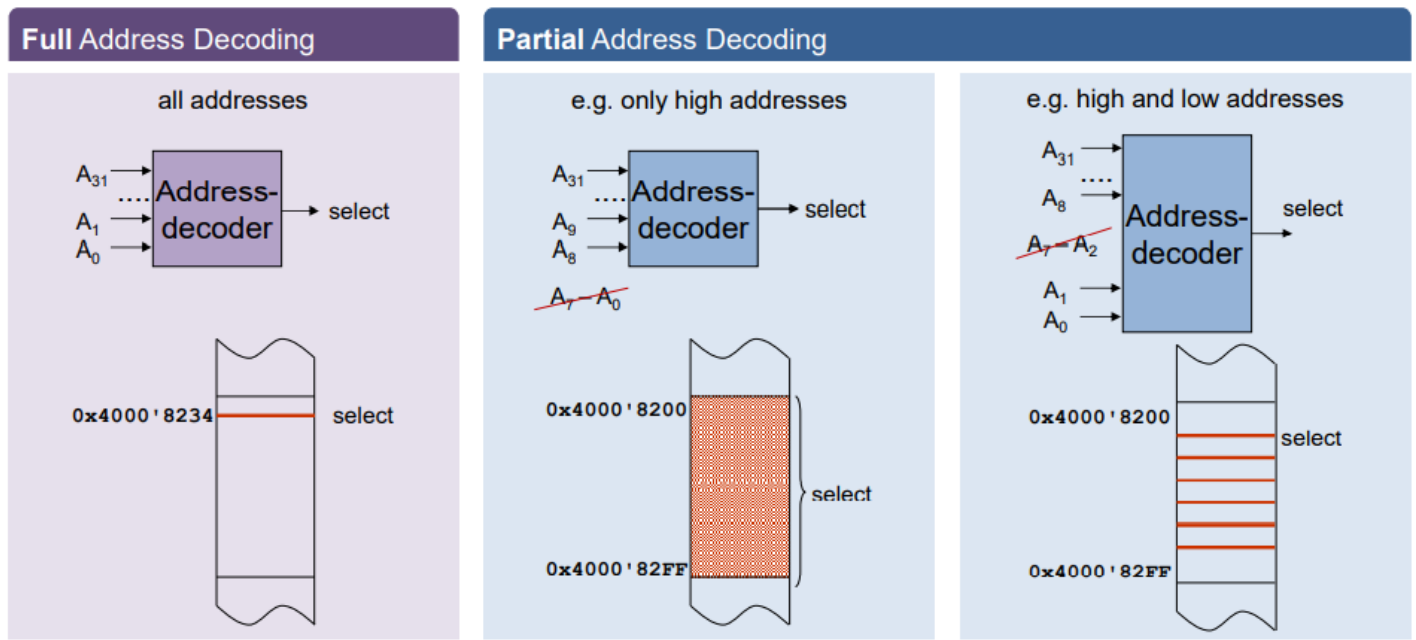
\includegraphics[width=\linewidth]{address_decoding.png}
\end{definition}